\documentclass[a4paper,12pt]{article}

\usepackage[
    left=2cm,
    right=2cm,
    top=3cm,
    bottom=3cm
]{geometry}

\usepackage[utf8]{inputenc}
\usepackage[czech]{babel}
\usepackage[T1]{fontenc}
\usepackage{graphicx}
\usepackage{array}
\usepackage{booktabs}
\usepackage{tabularx}
\usepackage{makecell}
\usepackage{float}
\usepackage{newunicodechar}
\usepackage{url}
\usepackage{siunitx}
\usepackage{listings}
\usepackage{xcolor}
\usepackage{diagbox}
\usepackage{hyperref}
\usepackage{tikz}
\usepackage{amsmath}
\usepackage{pgfplots}
\pgfplotsset{compat=1.18}

\usepackage{fancyhdr}
\pagestyle{fancy}

\fancyhf{}
\fancyhead[L]{Gamma spektrometrie}
\fancyhead[R]{Pavel Pernička}
\fancyfoot[C]{\thepage}

\fancypagestyle{firstpage}{
    \fancyhf{}
    \renewcommand{\headrulewidth}{0pt}
    \renewcommand{\footrulewidth}{0pt}
    \fancyfoot[C]{\thepage}
}

\definecolor{myblue}{RGB}{111,0,248}
\newcommand{\colorcircle}[1]{%
  \tikz[baseline=-0.6ex]\draw[fill=#1,draw=none] (0,0) circle (1.5ex);%
}
\newcommand{\unitC}{\,^\circ\mathrm{C}}
\newcommand{\unitV}{\,\mathrm{V}}
\newcommand{\unitA}{\,\mathrm{A}}
\newcommand{\units}{\,\mathrm{s}}
\newcommand{\unitmin}{\,\mathrm{min}}

\newcommand{\centered}[1]{\begin{tabular}{l} #1 \end{tabular}}

\addto\captionsczech{\renewcommand{\refname}{Seznam použité literatury}}
\addto\captionsczech{\renewcommand{\figurename}{\textbf{Obrázek}}}
\addto\captionsczech{\renewcommand{\tablename}{\textbf{Tabulka}}}
\renewcommand{\lstlistingname}{\textbf{Kód}}

\lstset{
    language=Python,
    basicstyle=\ttfamily\footnotesize,
    keywordstyle=\color{blue},
    commentstyle=\color{gray},
    stringstyle=\color{red},
    numbers=left,
    numberstyle=\tiny\color{gray},
    stepnumber=1,
    breaklines=true,
    frame=single
}

\begin{document}
\thispagestyle{firstpage}

\vspace*{\fill}
\begin{center}
\renewcommand{\arraystretch}{1.75}

\begin{tabularx}{\textwidth}{|X|X|X|}
    \hline
    \multicolumn{1}{|c|}{\rule{0pt}{2.25cm} 
\includegraphics[height=2cm]{img/ctu_logo.png}}
    & \multicolumn{2}{c|}{\makecell{\textbf{KATEDRA FYZIKY}}} \\
    \hline
    \multicolumn{3}{|c|}{\Large \textbf{\centered{LABORATORNÍ CVIČENÍ Z FEN}}} \\
    \hline
    \multicolumn{2}{|X}{\small{Jméno} \newline \textbf{Pavel Pernička}}
    & \multicolumn{1}{|X|}{\small{Datum měření} \newline \textbf{5.11.2025}} \\
    \hline
    {\small{Semestr} \newline \textbf{Zimní 2025}}
    & {\small{Ročník} \newline \textbf{2.}}
    & {\small{Datum odevzdání} \newline \textbf{16.1.2026}} \\
    \hline
    \multicolumn{3}{|c|}{\rule{0pt}{1cm}} \\
    \hline
    \multicolumn{1}{|X|}{\small{Číslo úlohy \newline \textbf{2}}}
    & \multicolumn{2}{|p{9cm}|}{\small{Název úlohy \newline \textbf{Gamma spektrometrie}}} \\
    \hline
\end{tabularx}

\end{center}
\vspace*{\fill}

\newpage
\section{Úkol měření}
\begin{itemize}
    \item Pomocí soustavy gamma spektrometru vytvořte spektrogramy radiačního pozadí a několika kalibračních vzorků.
    \item Ze spektrogramu vyčtěte, které zářiče jsme zachytili.
\end{itemize}


\section{Seznam použitých přístrojů}
\begin{itemize}
    \item Olověné stínicí bloky
    \item Scintilační gamma detektor na bázi vakuového fotonásobiče
    \item Zdroj vysokého napětí pro fotonásobič
    \item Předzesilovač signálu z fotonásobiče
    \item Tvaroveč signálu + multichannel analyzer
    \item Osciloskop pro sledování signálu
\end{itemize}

\section{Postup měření}
\begin{itemize}
    \item Nejprve změříme radiační pozadí tak, že vytáhneme scintilační detektor ze stínícího boxu, v ovládacím programu vymažeme spektrum, spustíme znovu měření a necháme několik minut běžet.
    \item Nyní provedeme podobným způsobem měření kalibračních vzorků $Na$ a $Co$, ale tentokrát uvnitř stínícího boxu, abychom odizolovali radiační pozadí.
\end{itemize}

\section{Fyzikální princip}
Atomové jádro má, podobně jako elektronový obal, diskrétní energetické stavy. Po radioaktivním rozpadu se dceřiné jádro často nachází v energeticky excitovaném stavu, který je nestabilní, a proto přechází do stavu s nižší energií. Tyto přechody probíhají pouze mezi povolenými hladinami a jsou doprovázeny emisí gamma fotonů, jejichž energie odpovídá rozdílu energií příslušných jaderných stavů a je charakteristická pro daný radionuklid.

Jako příklad můžeme uvést izotop \textsuperscript{60}Co, se kterým v této laboratorní úloze pracujeme. Tento radionuklid se rozpadá $\beta^-$ rozpadem na excitované jádro niklu:
\[
{}^{60}\mathrm{Co} \;\xrightarrow{\beta^-}\; {}^{60}\mathrm{Ni}^* + e^- + \bar{\nu}_e.
\]
Vzniklé jádro ${}^{60}\mathrm{Ni}^*$ se následně deexcituje do základního stavu pomocí dvou po sobě jdoucích přechodů, při nichž jsou emitovány dva gamma fotony:
\[
{}^{60}\mathrm{Ni}^* \rightarrow {}^{60}\mathrm{Ni} + \gamma_1 + \gamma_2,
\]
s charakteristickými energiemi
\[
E_{\gamma_1} = 1173\,\mathrm{keV}, \qquad E_{\gamma_2} = 1332\,\mathrm{keV}.
\]
Tyto energie bychom měli být schopni v naměřeném gamma spektru zachytit jako dva nepříliš vzdálené energetické peaky.


\section{Princip měření}

Pro zachycení a změření energie gamma fotonů využíváme jev zvaný scintilace. Při průchodu gamma záření scintilačním krystalem dochází k interakcím fotonů s látkou prostřednictvím fotoefektu nebo Comptonova rozptylu. 
takto předaná energie je ve scintilátoru částečně přeměněna na záblesk viditelného světla, jehož intenzita je úměrná energii absorbovaného gamma fotonu.

Vzniklé scintilační fotony jsou následně detekovány fotokatodou vakuového fotonásobiče (PMT), kde dochází k fotoelektrickému jevu a emisi elektronů. Ty jsou urychlovány a násobeny na soustavě dynod (díky přivedenému vysokému napětí), čímž vzniká krátký elektrický impuls s~amplitudou úměrnou počtu dopadajících scintilačních fotonů, a tedy i energii původního gamma fotonu. 
Tento impuls je dále zesílený a tvarovaný nízkošumovými přístroji.

Naměřená amplituda impulsu je přiřazena ke konkrétnímu kanálu vícikanálového analyzátoru, čímž vzniká energetické spektrum, které je vykresleno programem na počítači.

\begin{figure}[H]
\centering
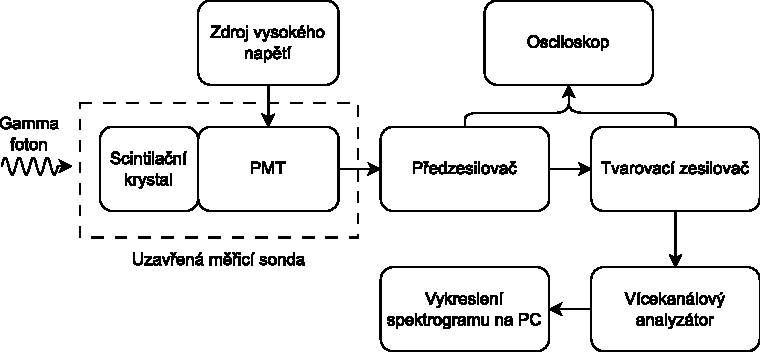
\includegraphics[width=\textwidth]{img/schema.pdf}
\caption{Schéma měřicí sestavy pro gamma spektrometrii}
\label{fig:chain}
\end{figure}


\newpage
\section{Naměřená spektra}
Pro vykreslení spekter použijeme data z vícekanálového analyzátoru, tedy počty zaznamenaných impulzů v jednotlivých energetických kanálech (binech), uložené ve formátu \textit{.spe}. Pro filtraci signálu a nalezení peaku použijeme program v jazyce python, který je součástí příloh.

\subsection{Kobalt 60}
Jedná se o výrazný zářič, na jehož spektrogramu\ref{fig:co_60_good} krásně vidíme dvojici peaků, která byla avizována v teoretickém úvodu. 
\begin{figure}[H]
\centering
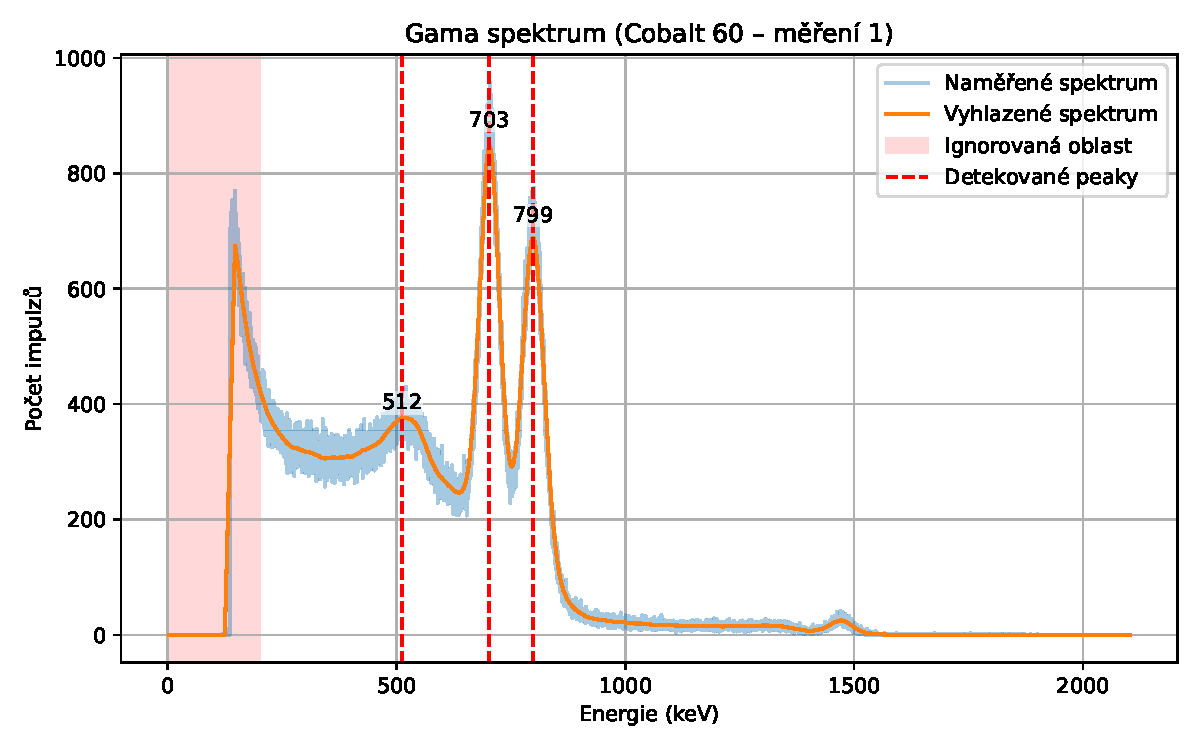
\includegraphics[width=0.90\textwidth]{img/charts/co60_v1_peaks.pdf}
\caption{Gamma spektrum Co 60 se stíněním, před kalibrací v softwaru}
\label{fig:co_60_precal}
\end{figure}

\begin{figure}[H]
\centering
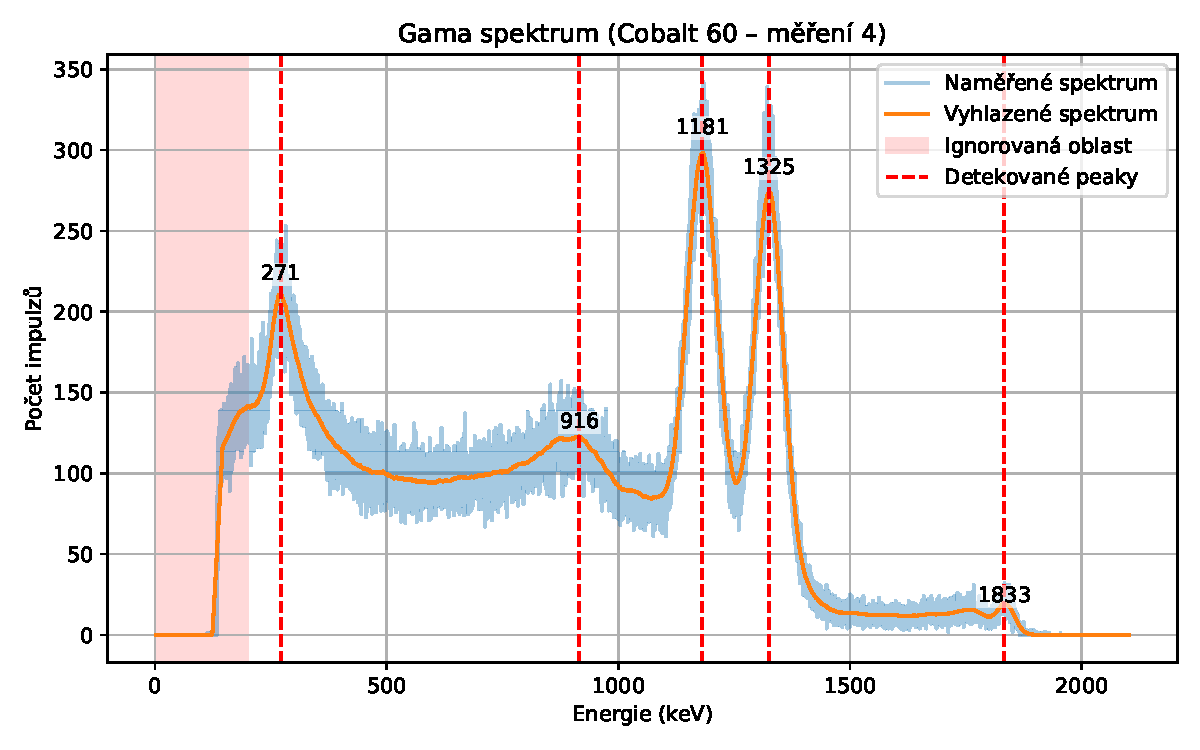
\includegraphics[width=0.90\textwidth]{img/charts/co60_v4_peaks.pdf}
\caption{Gamma spektrum Co 60 se stíněním, po správné kalibraci v softwaru}
\label{fig:co_60_good}
\end{figure}

\begin{figure}[H]
\centering
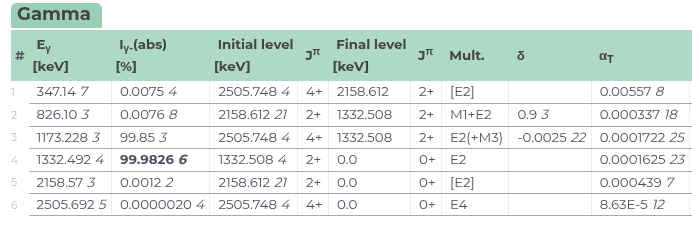
\includegraphics[width=0.90\textwidth]{img/iaea_co60_gamma.png}
\caption{Tabulkové hodnoty vyzářených fotonů pro Co 60}
\label{fig:co_60_tables}
\end{figure}

\subsection{Sodík 22}
Jelikož je sodíkový zářič slabější, než kobalková, můžeme na obrázcích \ref{fig:na_22_noshield} a \ref{fig:na_22_shield} vidět, jaký má vliv stínění na kvalitu měření. Na obrázku \ref{fig:na_22_shield} vidíme výrazný peak okolo $E_\gamma = 516\ keV$, který je dle tabulek způsoben anihalací pozitronu (vzniklého při $\beta -$ rozpadu Na 22 na Ne 22) s elektronem. Další peak $E_\gamma = 1203\ keV$ bude ten jediný v tabulce.
\begin{figure}[H]
\centering
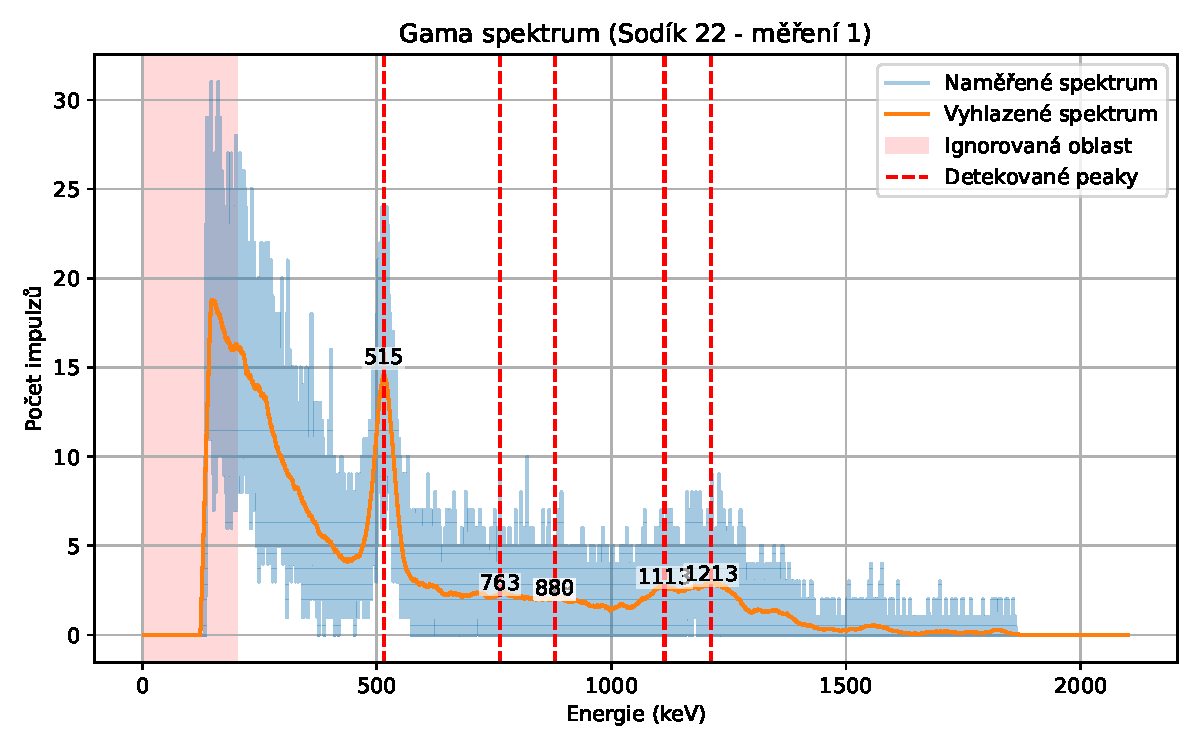
\includegraphics[width=0.90\textwidth]{img/charts/na22_final_peaks.pdf}
\caption{Gamma spektrum Na 22 bez stínění}
\label{fig:na_22_noshield}
\end{figure}

\begin{figure}[H]
\centering
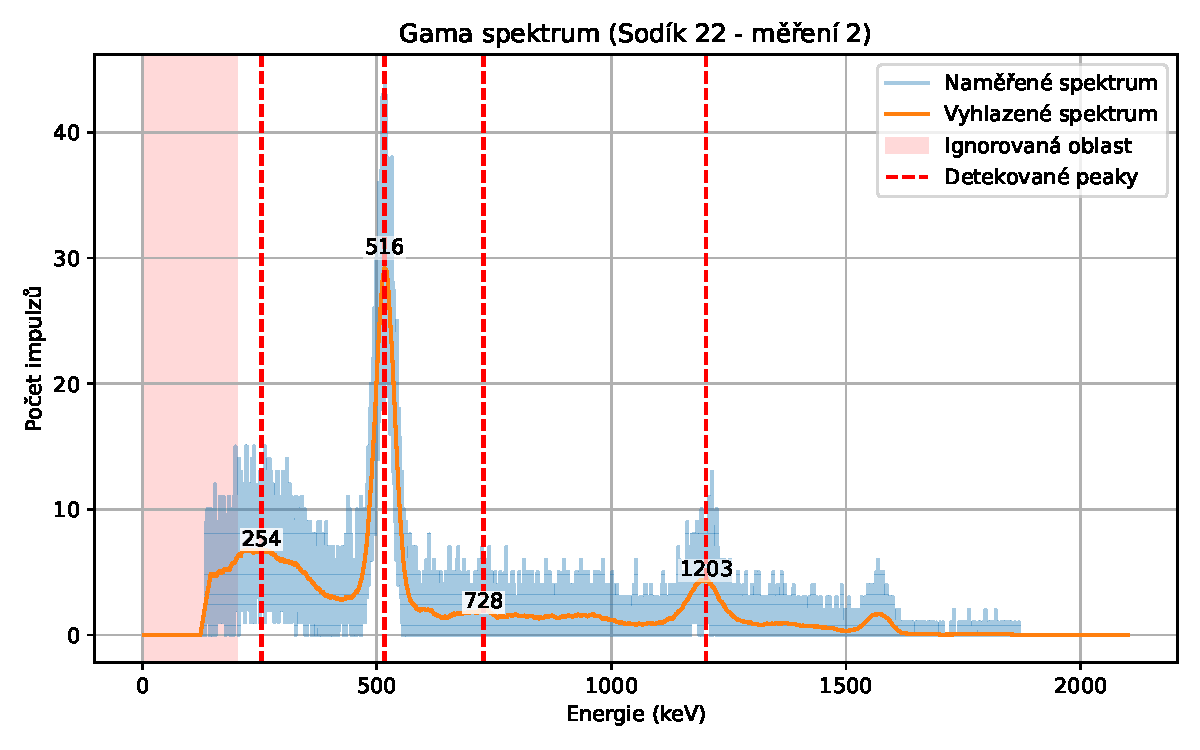
\includegraphics[width=0.90\textwidth]{img/charts/na22_stineny_peaks.pdf}
\caption{Gamma spektrum Na 22 se stíněním}
\label{fig:na_22_shield}
\end{figure}

\begin{figure}[H]
\centering
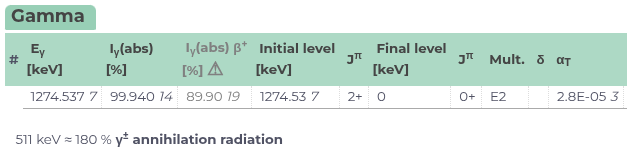
\includegraphics[width=0.90\textwidth]{img/iaea_na22_gamma.png}
\caption{Tabulkové hodnoty vyzářených fotonů pro Na 22}
\label{fig:na_22_tables}
\end{figure}

\subsection{Radiační pozadí}
U radiačního pozadí v obrázku \ref{fig:background} vidíme bohužel jen jeden výrazný peak s $E_\gamma=821\ keV$. Podle tabulek se může jednat buď o Co 58, který má $E_\gamma = 810,8\ keV$ nebo o Tl 208, které má $E_\gamma = 860,6\ keV$. Jelikož Tl 208 je součásti přirozené rozpadové řady Thoria, je prvděpodobné, že se jedná o něj.
\begin{figure}[H]
\centering
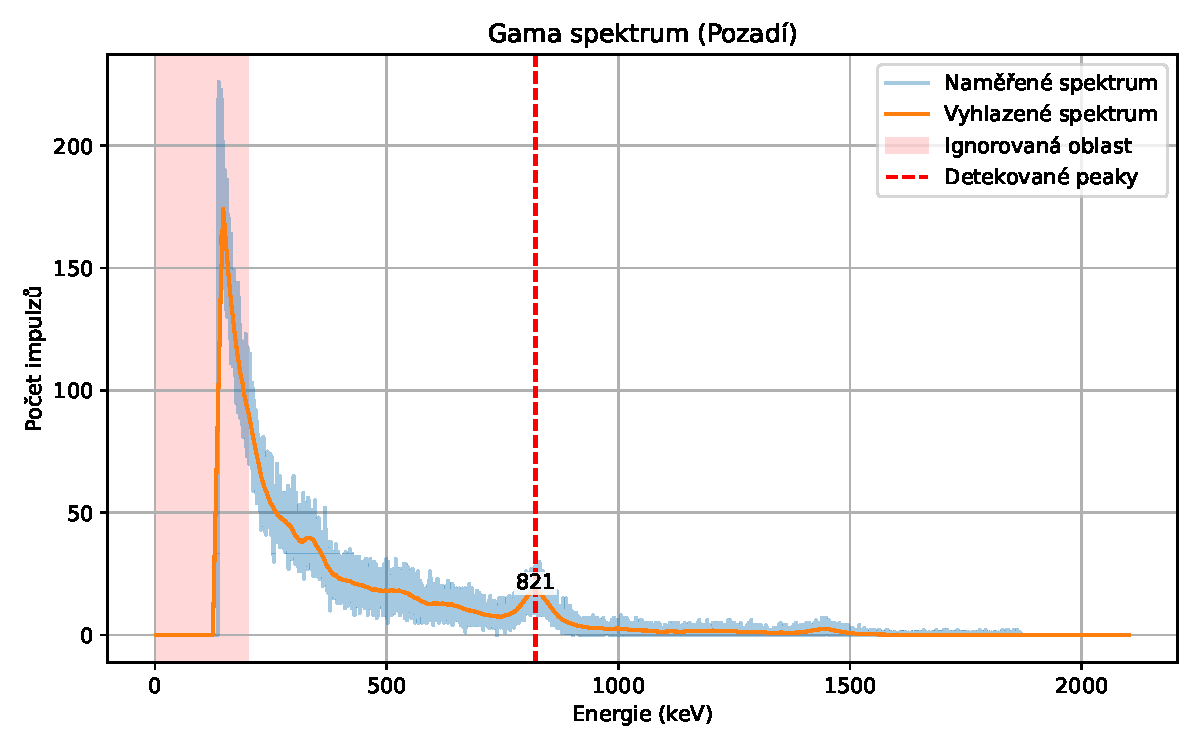
\includegraphics[width=0.90\textwidth]{img/charts/pozadi_1800s_peaks.pdf}
\caption{Gamma spektrum radiačního pozadí}
\label{fig:background}
\end{figure}

\newpage
\section{Závěr}
Pomocí laboratorní techniky jsme změřili gamma spektra kalibračních zářičů s izotopy Co 60 a~Na 22. Peaky ze spektrogramů jsme srovnali s tabulkovými hodnotami \cite{iaea} vyzářených fotonů s nejvyšší absolutní intenzitou $I_\gamma (abs)$ a tak jsme si křížově ověřili, že dostáváme správná data. V měření zejména u Na 22 máme větší nepřesnost peaků, protože jsme spektrum neměřili dostatečně dlouho a~tudíž nemáme tak ostrá maxima. 
V obrázku \ref{fig:na_22_shield} jde u očekávaného peaku $1264\ keV$ vidět, že by poměrně blízko k němu hodnoty dokonvergovaly.

\section{Přílohy}
\begin{itemize}
    \item Python skript pro vykreslení grafů a nalezení peaků z \textit{.spe} souborů.
    \item Naměřené spektrum ve formátu SPE
\end{itemize}

\begin{thebibliography}{}

    \bibitem{zadani}
    Jakub Cikhardt, Pavel Kubeš. \textit{Prezentace k předmětu Fyzika pro elektroenergetiku}. 2025.

    \bibitem{skripta}
    Michal Bednařík. \textit{Studijní texty k předmětu Fyzika 2}.
    
    \bibitem{iaea}
    International Atomic Energy Agency (IAEA). \textit{Live Chart of Nuclides}. Vienna. Dostupné online: \url{https://nds.iaea.org/relnsd/vcharthtml/VChartHTML.html}.


\end{thebibliography}

\end{document}
